% Generated by tex/build_swebok_structure.py from tex/chapters/ch01/05_要求分析.tex
\subsubsection{サービス品質制約の経済性}

サービス品質制約は、単に「高ければよい」ものではない。たとえば、応答時間を極限まで短くする、稼働率を極限まで高くする、処理能力を極限まで大きくするには、費用が増える。したがって、要求は価値と費用の関係で考える必要がある。

\term{失敗点}は、それを下回るとシステムとして価値がほとんどなくなる水準である。\term{完全点}は、それを超えても利用者に追加価値がほとんど出ない水準である。現実的には、要求値はこの間で決まる。最もよい水準は、価値と費用の差が最大になる点である。

\begin{figure}[htbp]
\centering
\IfFileExists{swebok_structure/CH01.ソフトウェア要求(Software_Requirements)/1.3.要求分析(Requirements_Analysis)/1.3.2.サービス品質制約の経済性(Economics_of_Quality_of_Service_Constraints)/assets/fig-ch01-07.png}{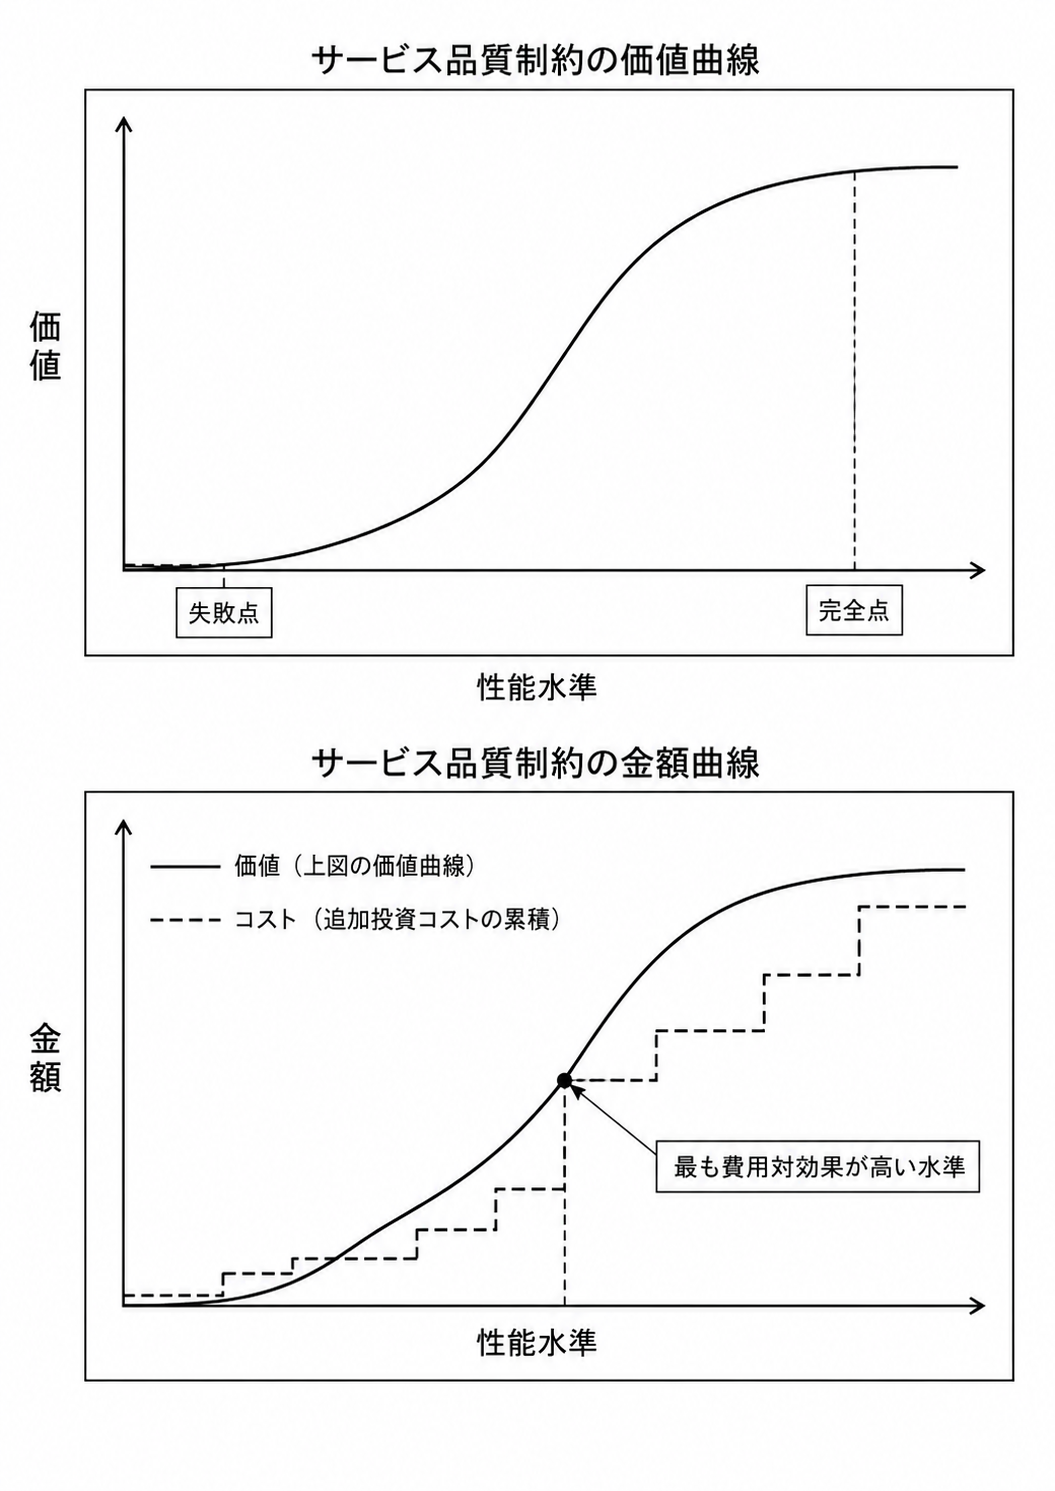
\includegraphics[width=0.96\linewidth]{swebok_structure/CH01.ソフトウェア要求(Software_Requirements)/1.3.要求分析(Requirements_Analysis)/1.3.2.サービス品質制約の経済性(Economics_of_Quality_of_Service_Constraints)/assets/fig-ch01-07.png}}{\fbox{\parbox[c][48mm][c]{0.9\linewidth}{\centering 画像生成待ち\\サービス品質制約の価値・費用曲線}}}
\caption{サービス品質制約の価値・費用曲線}
\label{fig:ch01-07}
\end{figure}

サービス品質制約同士には、よい関係と悪い関係がある。たとえば、コードを単純にすると信頼性と変更容易性が同時に上がることがある。一方、実行速度を極端に高める最適化が、コードを複雑にして変更容易性を下げることもある。
